% !TeX spellcheck = fr_FR
\section{\Pi{}}
En chinois, \Pi{} \begin{CJK*}{UTF8}{bsmi}劈\end{CJK*} signifie \textit{couper}, \textit{fendre}, \textit{aller droit vers}. En substance, \Pi{} est une coupe fendante.

En tant que technique de base, \Pi{} est simplement décrit comme une coupe verticale descendante. Elle est souvent associée à un moulinet intérieur ou extérieur que je ne décrirai pas ici puisqu'il ne fait pas strictement partie de la technique \Pi{} et aura plutôt sa place ailleurs.

Bien que la technique formelle \Pi{} soit dirigée vers le bas, je pense personnellement que l'énergie fendante de \Pi{} peut être orientée dans toute direction. Ainsi, même des coupes horizontales ou montantes qui fendent la cible de manière caractéristique sans aucun mouvement de trancher peuvent être en quelque sorte considérées comme affiliées à cette énergie.

La technique emblématique formelle \Pi{} se prépare en levant la poignée de l'épée à hauteur d'oreille pendant que l'on s'assied dans la jambe opposée à la main armée. La prise doit être relâchée mais fermement maintenue entre le majeur, l'annulaire et le pouce. Le contact relâché des autres doigts maintient un contrôle de la poignée tout en permettant une certaine flexibilité de la prise.
Dans un contexte moins formel et moins statique, on peut combiner cette préparation à un déplacement pendant une parade ou une esquive, dans une transformation continue de l'action défensive en riposte.

Dans la première phase de la coupe, la main est envoyée en diagonale et tire l'épée en avant vers le bas dans la direction du pommeau pour accélérer la lame. La force de biais exercée par la main sur la poignée entraîne ainsi graduellement la rotation de l'épée autour de son centre de gravité (fig. \ref{fig:pi_cut} a).

Ce mouvement tire son énergie de l'expansion du corps et le cas échéant d'un pas vers l'avant pour une portée plus importante et un gain de puissance.

Ensuite, dès que le centre de gravité a passé en avant de la main (fig. \ref{fig:pi_cut} b), celle-ci cesse d'exercer toute action et ne fait plus que suivre la poignée en maintenant simplement un contrôle relâché mais ferme de la trajectoire de l'épée. La lame se déplace ainsi librement avec une trajectoire non perturbée au moment où elle atteint la cible et toute l'énergie cinétique accumulée lors de la phase d'accélération est alors transférée dans la coupe (fig. \ref{fig:pi_cut} c).

\begin{figure}[ht]
\centering
	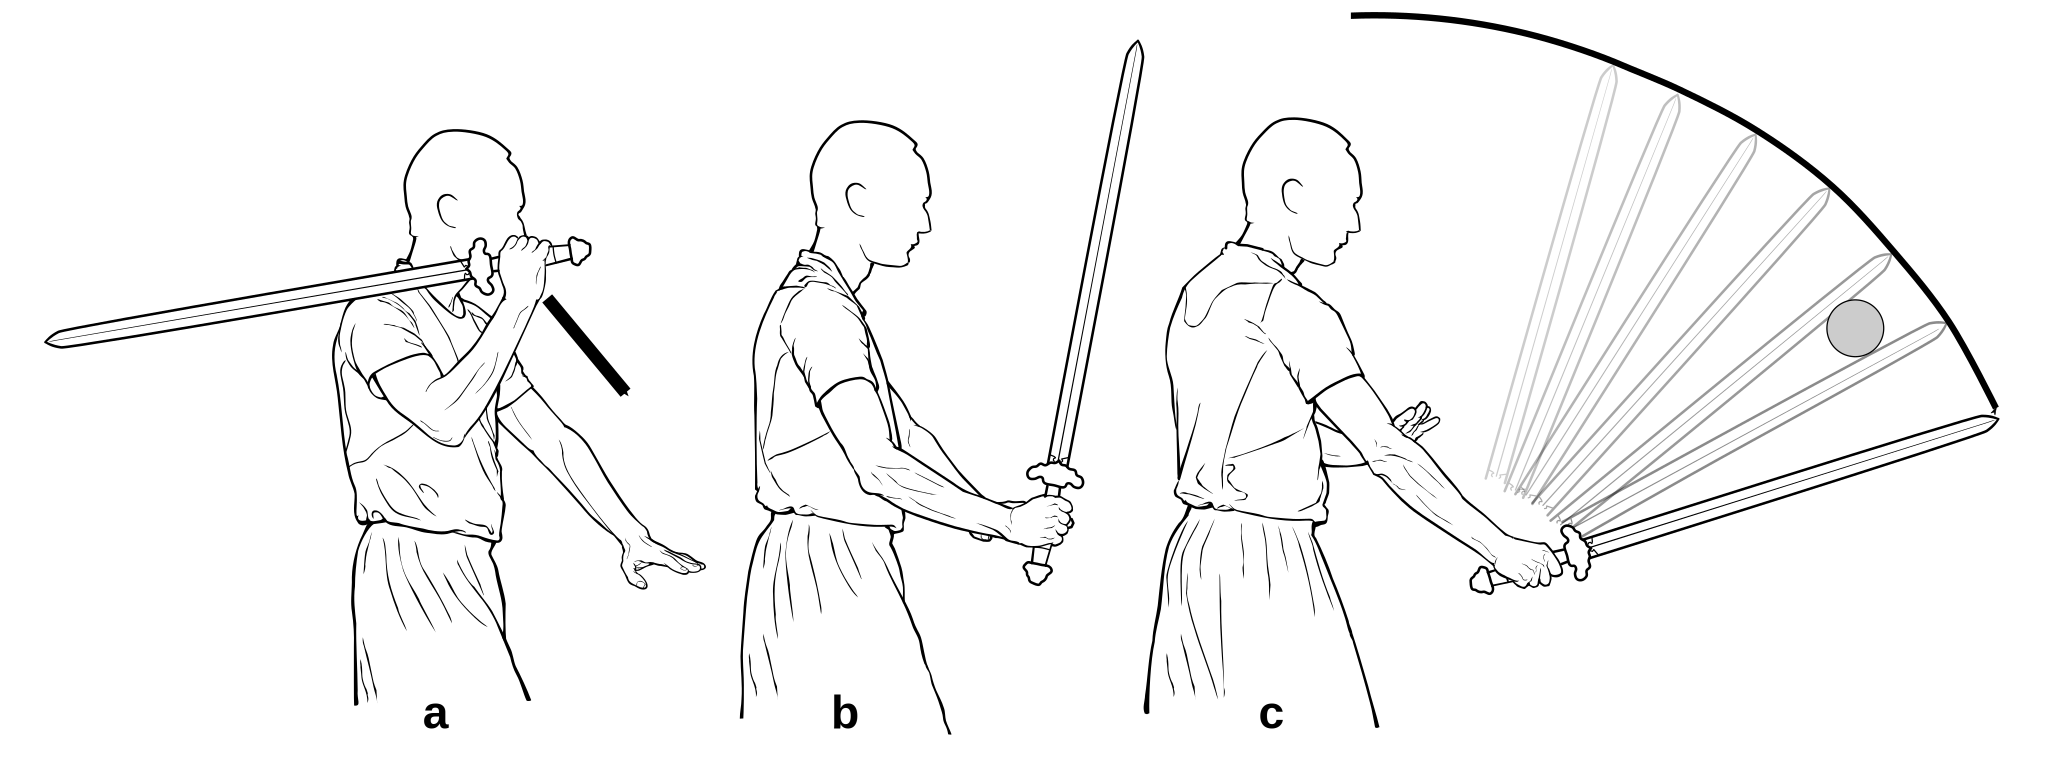
\includegraphics[width=1.00\textwidth]{../../Images/JibenJianfa/Pi/Pi_juxtaposed.pdf}
	\caption[Coupe \Pi{}]{Coupe \Pi{} : (a) Partant d'une position haute de l'épée, la main droite la tire vers le bas pour accélérer la lame; (b) montre la fin de la phase d'accélération, à partir de cet instant, la main n'exercera plus d'action sur la poignée; (c) la main suit la poignée avec juste un contrôle ferme de la trajectoire de l'épée de manière à ce que la lame puisse librement traverser la cible représentée par un cercle gris. Notez que la trajectoire de la pointe n'est pas un cercle mais un arc allongé.}
	\label{fig:pi_cut}
\end{figure}

Il est absolument indispensable que le plat de la lame soit parfaitement aligné avec la trajectoire de la l'épée pour garantir que le poids de la lame soit derrière le tranchant pour le pousser à travers la cible. Si jamais la lame atteignait la cible avec un angle, aussi petit soit-il, elle tendrait à tourner autour de son axe et pourrait rebondir dangereusement au lieu de trancher. Lorsque l'alignement est correct, au contraire, et que la prise est relâchée, la lame pourra traverser la cible de part en part sans retour notable.

Après la coupe, la poignée bute naturellement contre le talon de la main et les doigts resserrent leur prise pour arrêter l'épée dans une position de garde à hauteur de taille, sans aucune tension ni rebond. Grâce à une bonne structure corporelle, l'énergie de l'épée retourne ainsi au corps, aidant le recentrage, et la préparation de la technique suivante.